\documentclass[letterpaper]{article}
\usepackage{aaai}
\usepackage{times}
\usepackage{helvet}
\usepackage{courier}
\usepackage{algorithm}
\usepackage{url}
\usepackage[noend]{algorithmic}
\usepackage{amsmath}
\usepackage{amsfonts}
\usepackage{amssymb}
\usepackage{color}
\usepackage{subfig}
\usepackage{graphicx}




\pdfinfo{
/Title(Instance-Based Parameter Tuning and Learning for Evolutionary AI Planning)
/Subject (Proceedings of the )
/Author (AAAI)
}

\title{Instance-Based Parameter Tuning\\
for Evolutionary AI Planning }

\author{M{\'a}ty{\'a}s Brendel 
\and Marc Schoenauer \\ 
Projet TAO, INRIA Saclay \& LRI\\
Universit{\'e} Paris Sud\\
Orsay, France} 

\setcounter{secnumdepth}{0}
\begin{document}
\maketitle


\begin{abstract} \begin{quote}
Learn-and-Optimize ~(LaO) ~is ~a ~generic ~surrogate ~based method for parameter tuning combining learning and optimization. In this paper LaO is used to tune Divide-and-Evolve (DaE), an Evolutionary Algorithm for AI Planning. The LaO framework makes it possible to learn the relation between some features describing a given instance and the optimal parameters for this instance, thus it enables to extrapolate this relation to unknown instances in the same domain. Moreover, the learned model is used as a surrogate-model to accelerate the search for the optimal parameters. It hence becomes possible to solve intra-domain and extra-domain generalization in a single framework. The proposed implementation of LaO uses an Artificial Neural Network for learning the mapping between features and optimal parameters, and the Covariance Matrix Adaptation Evolution Strategy for optimization. Results demonstrate that LaO is capable of improving the quality of the DaE results even with only a few iterations. The main limitation of the DaE case-study is the limited amount of meaningful features that are available to describe the instances. However, the learned model reaches almost the same performance on the test instances, which means that it is capable of generalization. 
\end{quote}
\end{abstract}



\section{Introduction}

Parameter tuning is basically a general optimization problem applied off-line to find the best parameters for complex algorithms, for example for Evolutionary Algorithms (EAs). Whereas the efficiency of EAs has been demonstrated on several application domains \cite{practice08,ParameterSettingBook07}, they usually need computationally expensive parameter tuning. Consequently, one is tempted to use either the default parameters of the framework he is using, or parameter values given in the literature for problems that are similar to his one. 

Being a general optimization problem, there are as many parameter tuning algorithms as optimization techniques \cite{Eiben2007,Montero:2010}. However, several specialized methods have been proposed, and the most prominent today are Racing \cite{birattari2002}, REVAC \cite{Nannen07}, SPO \cite{SPO:CEC05}, and ParamILS \cite{ParamILS-JAIR}. All these approaches face the same crucial generalization issue: can a parameter set that has been optimized for a given problem be successfully used to another one? The answer of course depends on the similarity of both problems. However, even in an optimization domain as precisely defined as AI Planning, there are very few results describing meaningful similarity measures between problem instances. Moreover, until now, sufficiently precise and accurate features have not been specified that would allow the user to accurately describe the problem, so that the optimal parameter-set could be learned from this feature-set, and carried on to other problems with similar description. To the best of our knowledge, no design of a general learning framework with some representative domains of AI planning has been proposed, and no general experiments has been carried out yet in this direction.

In the SAT domain, however, one work must be given as an example of what can be done along those lines. In \cite{Hutter06}, many relevant features have been gathered based on half a century of SAT-research, and hundreds of papers. Extensive parameter tuning on several thousands of instances has allowed the authors to learn, using function regression, a meaningful mapping between the features and the running-time of a given SAT solver with given parameters. Optimizing this model makes it possible to choose the optimal parameters for a given (unknown) instance. The present paper aims at generalizing this work made in AI planning, with one major difference: the target will be here to optimize the fitness value for a given runtime, and not the runtime to solution -- as the optimal solution is generally not known for AI planning problems. The Learn-and-Optimize (LaO) framework consists of the combination of optimizing (i.e., parameter tuning) and learning, i.e., finding the mapping between features and best parameters. Furthermore, the results of learning will already be useful during further the optimization phases, using the learned model as in standard surrogate-model based techniques (see e.g., \cite{Bardenet} for a Gaussian-process-based approach).

LaO can of course be applied to any target optimization methodology that requires parameter tuning. In this paper, the target optimization technique is Evolutionary Algorithms (EA), more precisely the evolutionary AI planner called Divide-and-Evolve (DaE). However, DaE will be here considered as a black-box algorithm, without any modification for the purpose of this work than its original version described in \cite{BibEvoCop:2010}. 

The paper is organized as follows: AI Planning Problems and the classical YAHSP solver are briefly introduced in section \ref{section:planning}. Section \ref{section:dae} describes the evolutionary  Divide-and-Evolve algorithm. Section \ref{section:LaO} introduces the original, top level parameter tuning method, Learn-and-Optimize. The case study presented in Section \ref{section:results} applies LaO to DaE, following the rules of the International Planning Competition 2011 -- Learning Track. Finally, conclusions are drawn and further directions of research are proposed in Section \ref{section:conclusions}. 

\section{AI Planning}
\label{section:planning}

An Artificial Intelligence (AI) planning problem is defined by the triplet of an initial state, a goal state, and a set of possible actions. An action modifies the current state and can only be applied if certain conditions are met. A solution plan to a planning problem is an ordered list of actions, whose execution from the initial state achieves the goal state. The quality criterion of a plan depends on the type of available actions: in the simplest case (e.g. STRIPS domain), it is the number of actions; it may also be the total cost of the plan for actions with cost; and it is the total duration of the plan, aka {\em makespan}, for temporal problems with so called durative actions.

Domain-independent planners rely on the Planning Domain Definition Language PDDL2.1 \cite{Fox-JAIR-2003}. The history of PDDL is closely related to the different editions of the International Planning Competitions (IPCs \url{http://ipc.icaps-conference.org/}), and the problems submitted to the participants, written in PDDL, are still the main benchmarks in AI Planning.

The description of a planning problem consists of two separate parts usually placed in two different files: the generic domain on the one hand and a specific instance scenario on the other hand. The domain file specifies object types and predicates, which define possible states, and actions, which define possible state changes. The instance scenario declares the actual objects of interest, gives the initial state and provides a description of the goal. A state is described by a set of atomic formulae, or atoms. An atom is defined by a predicate followed by a list of object identifiers: (PREDICATE$\_$NAME $OBJ_1$ ... $OBJ_N$). 

The initial state is complete, whereas the goal might be a partial state. An action is composed of a set of preconditions and a set of effects, and applies to a list of variables given as arguments, and possibly a duration or a cost. Preconditions are logical constraints which apply domain predicates to the arguments and trigger the effects when they are satisfied. Effects enable state transitions by adding or removing atoms.

A solution plan to a planning problem is a consistent schedule of grounded actions whose execution in the initial state leads to a state that contains the goal state, i.e., where all atoms of the problem goal are true. A planning problem defined on domain $D$ with initial state $I$ and goal $G$ will be denoted in the following as ${\cal P}_D(I,G)$. 

\section{Divide-and-Evolve}

\label{section:dae}

Early approaches to AI Planning using Evolutionary Algorithms directly handled possible solutions. However, as it is often the case in Evolutionary Combinatorial optimization, those direct encoding approaches have limited performance in comparison to the traditional AI planning approaches. Furthermore, hybridization with classical methods has been the way to success in many combinatorial domains, as witnessed by the fruitful emerging domain of memetic algorithms \cite{MemeticBook:2005}. Along those lines, though relying on an original ``memetization'' principle, a novel hybridization of Evolutionary Algorithms (EAs) with AI Planning, termed Divide-and-Evolve (DaE) has been proposed \cite{DAE:EvoCOP06,DAE:book-2007}. For a complete formal description, see \cite{Bibai:ICAPS2010}.

The basic idea of DaE in order to solve a planning task ${\cal P}_D(I,G)$ is to find a sequence of states $S_1, \ldots, S_n$, and to use some embedded planner to solve the series of planning problems ${\cal P}_D(S_{k},S_{k+1})$, for $k \in [0,n]$ (with the convention that $S_0 = I$ and $S_{n+1} = G$). The generation and optimization of the sequence of states $(S_i)_{i \in [1,n]}$ is driven by an evolutionary algorithm. 
The fitness (quality criterion) of a list of partial states $S_1, \ldots,$ $S_n$ is computed by repeatedly calling the external 'embedded' planner to solve the sequence of problems ${\cal P}_D(S_{k},S_{k+1})$, $\{k=0,\ldots,n\}$. The concatenation of the corresponding plans (possibly with some compression step) is a solution of the initial problem. Any existing planner can be used as embedded planner, but since guarantee of optimality at all calls is not mandatory in order for DaE to obtain good quality results \cite{Bibai:ICAPS2010}, a sub-optimal, but fast planner is used: YAHSP \cite{V:icaps04} is a lookahead strategy planning system for sub-optimal planning which uses the  actions in the relaxed plan to compute reachable states in order to speed up the search process. 

A state is a list of atoms built over the set of predicates and the set of object instances. However, searching the space of complete states would result in a rapid explosion of the size of the search space. Moreover, goals of planning problem need only to be defined as partial states. It thus seems more practical to search only sequences of partial states, and to limit the choice of possible atoms used within such partial states. However, this raises the issue of the choice of the atoms to be used to represent individuals, among all possible atoms. The result of the previous experiments on different domains of temporal planning tasks from the IPC benchmark series \cite{BibEvoCop2009} demonstrates the need for a very careful choice of the atoms that are used to build the partial states. The method used to build the partial states is based on an estimation of the earliest time from which an atom can become true. Such estimation can be obtained by any admissible heuristic function (e.g $h^1,h^2...$ \cite{HaslumGeffner-AIPS-2000}). The possible start times are then used in order to restrict the candidate atoms for each partial state. A partial state is built at a given time by randomly choosing among several atoms that are possibly true at this time. The sequence of states is then built by preserving the estimated chronology between atoms (time consistency).

An individual in DaE is hence represented as a variable-length ordered time-consistent list of partial states, and each state is a variable-length list of atoms that are not pairwise mutex, as far as the initial grounding of all atoms  can tell (exactly determining if two atoms are mutex amounts to solving a complete planning problem). Furthermore, all operators that manipulate the representation (see below) maintain the chronology between atoms and the approximate local consistency of a state, i.e. avoid pairwise mutexes.

One-point crossover is used, adapted to variable-length representation in that both crossover points are independently chosen, uniformly in both parents.
Four different mutation operators have been designed, and once an individual has been chosen for mutation (according to a population-level mutation rate), the choice of which mutation to apply is made according to user-defined relative weights. 
Because an individual is a variable length list of states, and a state is a variable length list of atoms, the mutation 
operator can act at both levels: at the individual level by adding (addState) or removing (delState) 
a state; or at the state level by adding (addAtom) or removing (delAtom) some atoms in the given state. 
The list of DaE parameters that will be tuned in this paper is given in Table \ref{table:parameters}.


\section{Learn-and-Optimize for Parameter Tuning}
\label{section:LaO}

\subsection{The General LaO Framework}

As already mentioned, parameter tuning is actually a general global optimization problem, thus facing the routine issue of local optimality. But a further problem arises in parameter tuning, and this is the generality of the tuned parameters. Tuning only one instance has of course a sense if only that instance is to be solved. Parameters tuned for one instance however, may not be optimal for other instances, as \cite{BibGECCO:2010} demonstrates. Furthermore, this paper also demonstrates that parameter tuning for several domains simultaneously is even more difficult, if at all possible. Even when generalizing parameters learned on one instance to another instance of the same domain (intra-domain generalization) might be problematic, as there are instances with very different complexity in the same domain. The issue is of course even more critical when aiming at inter-domain generalization, i.e., learning the parameters on one or several instances, and using the learned parameters on instances of different domain than that of the training instances. Indeed, differences between the domains may cause a problem, and even instances of apparent similar complexity (e.g. same number of objects) may require different settings from domain to domain. The poor results with global tuning in \cite{BibGECCO:2010} indicate that these are issues to be considered. One workaround this generalization issue is to relax the constraint of finding a single universally optimal parameter-set, that certainly does not exist, and to focus on learning a complex relation between instances and optimal parameters. 

The proposed Learn-and-Optimize framework (LaO) aims at learning such relation, thus, in the ideal case, solving both the intra-domain and extra-domain generalization problems, by adding learning to optimization. The underlying hypothesis is that there exists a relation between some features describing an instance and the optimal parameters for solving this instance, and the goal of this work is to propose a general methodology to do so. If well designed, the features should describe differences both between instances from the same domain, and differences between instances of different domains -- and hence differences between domains, too. 
The case study analyzed here deals with AI planning, and some features extracted from both the domain-file and the instance-file will be proposed later.

Suppose for now that we have $n$ features and $m$ parameters, and we are doing per-instance parameter tuning on instance $\cal I$. For the sake of simplicity and generality, both the fitness, the features and the parameters are considered as real values. Parameter tuning is the optimization (e.g., minimization) of the fitness function (quality-criterion) \begin{math}f_{\cal I}:\mathbf{R}^m\to \mathbf{R} \end{math}, the expected value of the stochastic algorithm DaE executed with parameter \begin{math} p \in \mathbf{R}^m \end{math}. The optimal parameter set is defined by \begin{math} p_{opt}(I)=argmin_p\{f_{\cal I}(p)\} \end{math}. 

For each instance $\cal I$, consider the set \begin{math} F({\cal I}) \in \mathbf{R}^n \end{math} of the features describing this instance. 
Two relations have to be taken into account: each planning instance has features, and it has an optimal parameter-set. In order to be able to generalize, we have to get rid of the instance, and collapse both relations into one single relation between feature-space and parameter-space. By getting rid of the dependency to \cal I we get the relation as:

\begin{equation} p(F): \mathbf{R}^n \to \mathbf{R}^m, p(F)=p_{opt} \end{equation}	

Where both F and \begin{math}p_{opt}\end{math}  is taken for that instance $\cal I$ of which F belongs to. For the sake of simplicity let us assume that there exists an unambiguous mapping from the feature space to the optimal parameter space. However, we will indicate, if some problems in the results may be caused by an unambiguity. The relation \begin{math} p(F) \end{math} between features and optimal parameters can be learned by any supervised learning method capable of representing, interpolating and extrapolating  \begin{math}\mathbf{R}^n\to \mathbf{R}^m \end{math} mappings, provided sufficient data are available.

A simple method could be to use any standard parameter tuning method for an appropriate training set of instances in a given domain, and then to use an appropriate supervised learning method in order to learn the relationship between the features and the best parameters. However, learning and optimizing may be combined, and this is the main idea behind LaO. The idea of using some surrogate model in optimization is not new. Here, however, there are  several instances to optimize, and only one model is available, that maps the feature-space into the parameter-space. Nevertheless, there is no question about how to use such a model of \begin{math}p(F)\end{math} in optimization: one can always ask the model for hints about a given parameter-set. Of course, if the model were perfectly fit to the training data, it would be useless, since it would return the same hint as trained. Therefore under-fitting when learning the mapping from feature-space to parameter-space is beneficial during the optimization phase in order to get new hints. One shall of course also avoid the regular threat on learning algorithms, that is over-fitting. It seems reasonable that the stopping criterion of LaO is determined by the stopping criterion of the optimizer algorithm. After exiting one can also do a re-training of the learner with the best parameters found.

The proposed LaO algorithm is an open framework: one could use any appropriate learner for the mapping and any kind of optimizer for parameter tuning. LaO can of course be generalized to parameter tunning outside of AI planning. In most cases, where the parameters of an algorithm are to be tuned, there are instances of application, and in each of these cases, there is a possibility to improve the tuning by also learning the relation between some features and the optimal parameters.



\subsection{An Implementation of LaO}

A simple multilayer Feed-Forward Artificial Neural Network (ANN) trained with standard backpropagation was chosen here for the learning of the features-to-parameters mapping, though any other supervised-learning algorithm could have been used. The implicit hypothesis is that the relation \begin{math}p(F)\end{math} is not very complex, which means that a simple ANN may be used. In this work, one mapping is trained for each domain. Training a single domain-independent ANN is left for future work.

The other decision for LaO implementation is the choice of the optimizer used for parameter tuning. Because parameter optimization will be done successively for several instances, the simple yet robust (1+1)-Covariance Matrix Adaptation Evolution Strategy \cite{hansen2001ecj}, in short CMA-ES,  was chosen, and used with its robust own default parameters. The advantage of CMA-Es is that it does not need derivatives -- which we do not have -- yet it tries to estimat a natural gradient with only a small amount of computational time.

One original component, though, was added to some direct approach to parameter tuning: gene-transfer between instances. There will be one (1+1)-CMA-ES running for each instance, because using larger population sizes for a single instance would be far too costly. However, the (1+1)-CMA-ES algorithms running on all training instances form a population of individuals. The idea of gene-transfer is to use some 'crossover'-like mechanism between the individuals of this population. Of course, the optimal parameter sets for the different instances are different; However, a good 'chromosome' of one instance may at least help another instance. Thus it may be used as a hint in the optimization of that other instance. Therefore random gene-transfer was used in the present implementation of LaO, by calling the so-called {\em Genetransferer}. When the Genetransferer is requested for a hint for one instance, it returns with uniform random distribution the so-far best parameter of a different instance (preventing, of course, that the default parameters are tried twice). Another benefit from gene-transfer is that it may smoothen out the ambiguities between instances, by increasing the probability for instances with the same features to test the same parameters, and thus the possibility to find out that the same parameters are appropriate for the same features. Algorithm 1 shows the pseudo-code of the resulting LaO.

\vspace{-0.2cm}
\begin{algorithm}[h!]
\caption{learn-and-optimize()}
\label{algolao}
{\small
\begin{algorithmic}[1]
\REQUIRE{\#cma, \#epochs, instances }
\WHILE{exitCriterionFalse()}
\FOR{$c=1 \to \#cma$}
\FORALL{$I \in instances$}
\STATE $p \gets I.callCMA()$ //each instance has its own CMA
\STATE $f \gets I.evaluate(p)$ //also keeping track of best p
\STATE $I.updateCMA(f)$
\ENDFOR
\STATE $c \gets c + 1$
\ENDFOR
\FORALL{$I \in instances$}
\STATE $I^* \gets callGenetransferer(I)$ //a different instance
\STATE $p \gets I^*.getBestParameter()$
\STATE $f \gets I.evaluate(p)$
\ENDFOR
\FORALL{$I \in instances$}
\STATE $p \gets I.getBestParameter()$
\STATE $F \gets I.getFeatures()$
\STATE $addANN(F,p)$
\ENDFOR
\STATE $trainANN(\#epochs)$
\FORALL{$I \in instances$}
\STATE $F \gets I.getFeatures()$
\STATE $p \gets callANN(F)$
\STATE $f \gets I.evaluate(p)$
\ENDFOR


\ENDWHILE
\RETURN{} 
\end{algorithmic}
}
\end{algorithm}
\vspace{-0.2cm}

Care must be taken when using the ANN and the Genetransferer as external hints within the standard CMA-ES process, to avoid corrupting it. CMA-ES should be informed about the external hints, if they improve the fitness-function. The proposed solution is to handle them as if they were the hint of the CMA-ES algorithm, i.e. to replace a standard request from CMA-ES by the value of the external hint, thus minimizing possible corruption. The global step size is updated with true or false, depending on the improvement or lack of improvement, and as in the usual CMA-ES algorithm, the covariance matrix is updated only in the later case.

\begin{table*}[ht]
\centering
\begin{tabular}{l c c c c c c c}
\hline\hline
Domain & \# of & \# training & \# test &  ANN & quality-ratio & quality-ratio & quality-ratio \\ 
Name & iterations  & instances &  instances &  error & in LaO & ANN on train & ANN on test \\ 
\hline
Freecell& 16 & 108 & 230 & 0.1 & 1.09 & 1.05 & 1.04  \\
Grid & 10 & 55 & 124 & 0.09 & 1.09 & 1.05 & 1.03  \\
Mprime & 8 & 64 & 152 & 0.08 & 1.11 & 1.05 & 1.04   \\
\hline
\end{tabular}
\caption{Results by domains (only the actually usable training instances are shown). ANN-error is given as MSE, as returned by FANN. The quality-improvement ratio in Lao is that of the best parameter-set found by LaO.}
\label{table:domains}
\end{table*} 


One additional technical difficulty arose with CMA-ES: each parameter is here restricted to an interval. This seems reasonable and makes the global algorithm more stable. Hence the variables of the search-space of the optimizer are actually normalized linearly onto the [0,1] interval. It is hence possible to apply a simple version of the box constraint handling technique described in \cite{hansen2009tec}, with a penalty term simply defined by \begin{math}||p^{feas}-p|| \end{math}, where \begin{math}p^{feas}\end{math} is the closest value in the box, i.e. the orthogonal projection to the border. Moreover, only \begin{math}p^{feas}\end{math} was recorded as a feasible solution , and later passed to the ANN. Note that the GeneTransferer and the ANN itself cannot send hints outside of the box. In order to not to compromise too much CMA-ES, several iterations of this were carried out for one hint of the ANN and one gene-transfer.

The implementation of LaO algorithm uses the Shark library \cite{shark08} for CMA-ES and the FANN library for ANN \cite{nissen}. To evaluate each parameter-setting with each instance,  a cluster was used, that has approximately 60 nodes, most of them with 4 cores, some with 8. However, this cluster is used by many researchers, therefore our algorithm was automatically scheduled to only use the spare CPU cycles on this cluster. Because of the heterogeneity of the hardware architecture used here, it is not possible to rely on accurate predicted running times. Therefore, for each evaluation, the number of YAHSP evaluations is fixed for DaE. Note that the number of YAHSP evaluations is approximately proportional to the running time, so that the execution time for a particular computer is also determined independently of the parameter-settings. For example, even if the size of the population is increased, because of the fixed number of evaluations that is allowed, the number of generations will be limited accordingly in order to approximatively allow the same running time for each parameter-setting optimization. Moreover, since DaE is not deterministic, 11 independent runs were carried out for each DaE experiment with a given paramter-set, and the fitness of this parameter set was taken to be the median fitness-value obtained by DaE.




\section{Results}
\label{section:results}

In the Planning and Learning Part of IPC2011 (IPC), 5 sample domains were pre-published, with a corresponding problem-generator for each domain: Ferry, Freecell, Grid, Mprime, and Sokoban. Ferry and Sokoban were excluded from this study since there were not enough number of instances at hand to learn any mapping. For each of the remaining 3 domains, 100 instances were generated, since this seemed to be appropriate for a running time of approximately 2-3 weeks: The competition track description fixes running time as 15 minutes. For each instance, 11 independent trials were run on a dedicated server to measure the median of number of evaluations with our default parameters. The termination criterion was the number of YAHSP evaluations. The median of those 11 runs were used as a termination criterion for each instance in the train set on any computer afterwards. However, many instances were never solved within 15 minutes, and those instances were dropped from the rest of experiment. The remaining instances were used for training.

Table \ref{table:domains} shows the data for each domain, as you can see from the approximately 100 instances from each domain we could not always make use of all training instances, except in the Freecell domain (108). In the other domains the more complex instances could not be solved in 15 minutes on the dedicated server. 

Table \ref{table:domains} also shows information about results. The Mean Square Error (MSE) of the retrained ANN is shown for each domain. Note that since there can be multiple optimal parameters for the same instance (fitness-function is discrete), there might be an unavoidable error of the ANN. 5 iterations of CMA-ES were carried out, followed by one ANN and one Genetransferer, and this cycle was iterated in the algorithm. This means that for example for the Grid domain LaO was running for 10 iterations and CMA-ES was called 50 times in total. One has to note that this is not much, but we were restricted by time. The ANN had 3 fully connected layers, and the hidden layer had the same number of neurons as the input. Learning was done by the conventional back-propagation algorithm, which is the default in FANN. In one iteration of LaO the ANN was only trained once for 50 iterations (called epochs in FANN) without reseting the weights, so that we avoid over-training. The aim of not reseting the weights was that the ANN makes a graded transition from the previous best known parameter-set to the new best known parameter-set, which could help optimization by trying some intermediate values. This means that over the 10 iterations of LaO in the domain Grid 500 iterations (epochs) of the ANN were carried out in total. However, note that the best parameters were trained with much less iterations, depending on the time when they were found. In the worst case, if the best parameter was found in the last iteration of LaO, it was trained for only 50 epochs and not used anymore, only recorded in the logs. This is why retraining is needed in the end.

 \begin{table}[tb!]
\centering
\begin{tabular}{l c c c c c c}
\hline\hline
Name & \ Default & \ CMA-ES &  Transferer & ANN \\ 
\hline
Freecell & ~0 -- ~9& 64 -- 66  & 18 -- ~8  & 18 -- 17     \\
Grid & ~2 -- 24 & 66 -- ~60  & 16 -- 11 & 17 -- ~5  &    \\
Mprime &  ~2 -- 45& 59 -- 36 & ~2 -- 11  & 18 -- ~8  &    \\
\hline
\end{tabular}
\caption{The share of the different sub-algorithm in finding the optimal parameters. For each sub-algorithm (Default, CMA-ES, Transferer=Genetransferer or ANN), the percentage of instances on which this method gave the best parameter set. Each cell shows 2 figures: the first one considers all occurrences of a method, no matter if another method also leads to an equivalent parameter set, as good as the first one. The second figures only consider the first method (from left to right) that discovered the best parameter-set.}
\label{table:hints}
\end{table} 

\begin{table}[ht]
\centering
\begin{tabular}{l c c c}
\hline\hline
Name & Min & Max & Default \\ 
\hline
Probability of crossover & 0.0 & 1 & 0.8 \\
Probability of mutation & 0.0& 1& 0.2 \\
Rate of mutation add station& 0& 10& 1 \\
Rate of mutation delete station& 0& 10& 3 \\
Rate of mutation add atom& 0& 10& 1 \\
Rate of mutation delete atom& 0& 10& 1 \\
Mean average for mutations& 0.0& 1& 0.8 \\
Time interval radius& 0& 10& 2 \\
Maximum number of stations& 5& 50& 20 \\
Maximum number of nodes& 100& 100 000& 10 000 \\
Population size& 10& 300& 100 \\
Number of offspring & 100& 2 000& 700 \\
\hline
\end{tabular}
\caption{DaE parameters that are controlled by LaO}
\label{table:parameters}
\end{table} 


 \begin{table*}[ht]
\centering
\begin{tabular}{l c c c c }
\hline\hline
Domain &\# goals & \# fluents  & \# objects  & mutexdensity   \\ 
\hline
Freecell & 2 & [28,34] 31.17, 1.68  & [32, 38] 35.17, 1.68  & [0.14, 0,17] 0.15, 0.005     \\
Grid & [7,9] 8, 1  & [58,59] 74.07, 9.38 & [56,90] 72.07, 9.38  & [0.08, 0.1] 0.09, 0.009     \\
Mprime & [8,9] 9, 1 & [32,40] 36, 2.09  & [42,52] 47, 2.009 & [0.03 0.03] 0.03, 0     \\
IPC6 all& [1,110] 23.32, 19.2 & [4,217] 30.6, 25.5  & [7,301] 45.2, 35.16  & [0,0.48] 0.1, 0.07     \\
\hline
\end{tabular}
\caption{Statistics of some features per domains in the train-set. Values given are [min,max] average, standard deviation respectively. If a feature is constant, one number is given.}
\label{table:statistics}
\end{table*} 

A parameter-set in LaO may come from different sources, namely it can be the default parameter-set, or requested from the CMA-ES, the Genetransferer or the ANN. It is an important information to know how good these sources work in optimization. Table \ref{table:hints} serves this purpose: it shows the share of the sub-algorithms in finding the optimal parameter-set in LaO, i.e. how each source contributes to the best parameter-settings in the end. For each source the first number shows the ratio the source contributed to the best result if tie-breaks are taken into account, the second number shows the same, if only the first best parameter-set is taken into account. Note that the order of the sources is as it is in the table: for example if CMA-ES found a different parameter-settings with the same fitness as the default, that is not included in the first ratio, but it is included in the second. Analyzing both numbers can lead to interesting conclusions. For example, for domain Mprime the default parameter-settings was the optimal for 45\% of the instances, however, only in 2\% of the instances there was no other parameter-setting found with the same quality. In the domain Freecell, the share of ANN is quite high (18\%), moreover we can see that in most of the cases the other sources did not find a parameter-set equally good (17\%). While Genetransferer in Freecell take equal share (18\%) of all the best parameters, but only a part of them (8\%) were unique. Note that CMA-ES was returning the first hint in each iteration and had 5 times more possibilities than the ANN. Taking this into account both the ANN and Genetransferer made an important contribution to optimization.

Termination criterion in the competition was simply the available time, the algorithm was running for several weeks on our cluster, which is used also for other research, i.e. only a small number of 4 or 8-core processors were available for each domain in average. After stopping LaO, retraining was made with 300 ANN epochs with the best data, because the ANN's saved directly from LaO may be under-trained. The MSE error of the ANN did not decrease using more epochs, which indicates that 300 iterations are enough at least for this amount of data and for this size of the ANN. Tests with 1000 iterations did not produce better results and neither training the ANN uniquely with the first found best parameters.


The controlled parameters of DaE are described in table \ref{table:parameters}. For a detailed description of these parameters, see \cite{BibGECCO:2010}. The feature-set consists of 12 features. First there are 5 important features: the number of fluents, goals, predicates, objects and types. These were extracted from the domain file or the instance file using the PDDL parser. One further feature we think could even be more important is called mutex-density, which is the number of mutexes divided by the number of all fluent-pairs. We also kept 6 less important features: number of lines, words and byte-count - obtained by the linux command "wc" - of the instance and the domain file. These features were kept only for historical reasons: they were used in the beginning as some "dummy" features. 



\begin{figure}[h!]
  \centering
    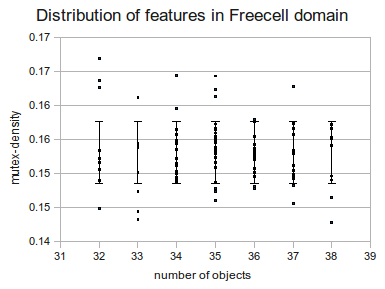
\includegraphics[width=0.5\textwidth]{results/freecell_train_objects_mutex-density.png}
  \caption{Distribution of the features "number of objects" and "mutex-density" in train-set in Freecell domain. One dot represents one problem, error-bars show standard deviation.}
\label{figure:featuresdistribution}
\end{figure}

Table \ref{table:statistics} shows some statistical properties of some selected features for each domain. Most of the features were correlated with each other, like \#objects, \#fluents, \#goals and also the wc-features. This means that actually we do not have much information on the input-side. Mutex-density is good, because it is independent of the other features, as it is shown in figure \ref{figure:featuresdistribution}. You can see that we have all kind of mutex-densities regardless of the number of objects. Standard-deviation-boxes look also the same for each value of number of objects.


\begin{figure}[h!]
	\centering
	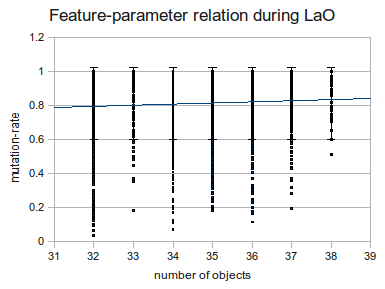
\includegraphics[width=0.5\textwidth]{results/freecell_lao_objects_mutrate.png}
	\caption{Relation between the feature "number of objects" and the parameter "mutation rate" in LaO, in the train-set in Freecell domain. Values of 		"mutation rate" are the optimal values found by LaO. This looks bad, but not unexpected. We can explain this. It is however questionable to show 		it. Error-bars-show standard deviation.}
	\label{figure:laoobjectmutrate}  
\end{figure}


\begin{figure}[h!]
	\centering
	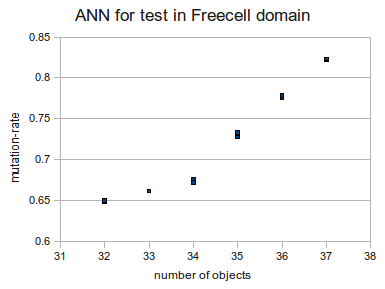
\includegraphics[width=0.5\textwidth]{results/freecell_test_objects_mutrate.png}
	\caption{Relation between the feature "number of objects" and the parameter "mutation rate" as learned by the ANN, during evaluation on the test-set in Freecell domain.}
	\label{figure:ANNobjectmutate}  
\end{figure}


Figure \ref{figure:laoobjectmutrate} shows the optimal parameter-values for mutation-rate and the feature ``number of objects'' for each training instance in the domain Freecell after terminating. Figure \ref{figure:ANNobjectmutate} shows for the trained ANN the same feature and parameter for the test-instances. We can see here what kind of model we get after training on the data produced by LaO. Note that these figures are the projection of the multidimensional feature- and parameter-space. The seeming unambiguity can have several explanations: (i) other features may be involved in the relation (ii) LaO was executed for a short time, therefore the relation is far from the real, optimal parameter-sets (iii) the feature-set is too weak to resolve an unambiguity. Nevertheless, the ANN seems to 'cut through': it reduces the relation as shown in the figure and this is acceptable.

Since testing was also carried out on the cluster, the termination criterion for testing was also the number of evaluations fixed for each instance. For evaluation the quality-improvement (quality-ratio) metric as used in IPC competitions. As a baseline we took the default parameter-setting. The ratio of the fitness value for the default parameter and the tuned parameter was computed and average was taken over the instances in the train or test-set. 

\begin{equation}Q=\frac{Fitness_{baseline}}{Fitness_{tuned}}\end{equation}

Note that since our termination criterion is number of evaluations, there was no unsolved instance. If an instance was unsolvable with default parameters within the specified time, it was dropped. 

Table \ref{table:domains} also presents several quality-improvement ratios. Label "in LaO" means that the best found parameter is compared to the default. By definition this ratio can not be less than 1 for any instance. We also present quality-improvement ratios for the retrained ANN on the training-set and the test-set. In these later cases, numbers less then 1 are possible, but were rare. As it can be seen we achieved a considerable quality-gain in training, but the transfer of this improvement to the ANN-model was only partial. Reasons for this may be different. First, there is the unambiguity of the mapping, second, the ANN may not be complex enough for the mapping, but most probably the feature-set is not powerful enough. On the other hand, the ANN model generalizes excellently to the independent test-set. Quality-improvement ratios dropped only by 0.01, i.e. the knowledge incorporated in the ANN was transferable to the test cases and usable almost to the same extent as for the train set. Our results are quite similar for each domain. Even the size of the training set seems not to be so crucial. For example for Freecell all the instances (108 out of 108 generated) could be used, because they were not so hard. On the other hand, only few  Grid instances (55 out of 107 generated) could be used. However, both performed well. The explanation for this may be that both the 32 and 108 instances covered well the whole range of solvable instances.

\section{Conclusions and Future Work}
\label{section:conclusions}
\label{section:futurework}	

Our method presented in this paper is a surrogate-model based combined learner and optimizer for parameter tuning. We demonstrated that our algorithm is capable of improving the quality of the DaE algorithm considerably even with only a few iterations. An appropriate number of iterations, like 1000 shall be carried out to demonstrate the capability of the algorithm. We also demonstrated that some of this quality-improvement can be incorporated into an ANN-model, which is also able to generalize excellently to an independent test-set.

Since LaO is only a framework, as indicated other kind of learning methods, and other kind of optimization techniques may be incorporated. If an ANN is used, the optimal structure has to be determined, or a more sophisticated solution is to apply one of the so-called Growing Neural Network architectures. Also the benefit of gene-transfer and/or cross-over might be investigated further. Gene-transfer shall be improved so that chromosomes are transfered deterministically in order of similarity of instances measured by similarity of features. One shall also test how inter-domain generalization works. It might be possible to learn a mapping for all domains, since the features may grasp the specificity of a domain. The present results indicate that the current feature set is too small and should be extended for better results. Feature-selection would become important only if the number of features is large compared to the number of examples. Unfortunately, this is not the case yet.


\section{Acknowledgements}
This work is funded through French ANR project DESCARWIN ANR-09-COSI-002.
% \section{Restrictions on Further Use}


\bibliographystyle{aaai}
\bibliography{icaps2011}
\end{document}






